\documentclass[11pt, handout]{beamer}
\usepackage[utf8]{inputenc}
\usepackage{datetime}
\usepackage{amsmath}
\usepackage{amssymb}
\usepackage{amsthm}
\usepackage{bbm}
\usepackage{bm}
\usepackage{hyperref}
\usepackage{environ}
\usepackage{mathrsfs}
\usepackage{mathtools}
\usepackage{tikz}

\usetheme{CambridgeUS}
\usecolortheme{default}

\newcommand\Fontvi{\fontsize{10}{12}\selectfont}
\newcommand\Fontvii{\fontsize{9}{10}\selectfont}

\setbeamertemplate{theorems}[numbered]
\newtheorem{proposition}{Proposition}

\newcommand{\circled}[1]{%
  \scalebox{0.6}{\tikz\node%
    [outer sep=0pt, inner sep=2pt,
      line width=0pt,text=white,fill=blue!50,draw,circle,shading=ball]{#1};%
  }%
}
\newcommand{\bref}[1]{\circled{\ref{#1}}}

\newdate{date}{31}{01}{2022}

\title[Lijoi et al. (2007)]{Bayesian nonparametric estimation of the probability of discovering new species}
\subtitle{Lijoi, Mena \& Pr{\"u}nster (2007)}
\author{Stefano Cortinovis}
\date[20605 - Machine Learning II]{\displaydate{date}}

% \AtBeginSection[]
% {
%     \begin{frame}
%         \frametitle{Table of Contents}
%         \tableofcontents[currentsection]
%     \end{frame}
% }

\begin{document}

\nocite{*}

\begin{frame}
\titlepage
\end{frame}

\section{Species sampling}

\begin{frame}[t]{Species sampling framework}
We formalize the process of drawing samples from a large population of individuals that can be grouped in different species as follows:
\begin{itemize}
    \item Let \((X_n)_{n \geq 1}\) be a sequence of random variables taking values in some set \(\mathbb{X}\).
    \begin{itemize}
        \item \(X_n\) represents the \textbf{species} of the \(n\)-th individual sampled
        \item \(\mathbb{X}\) represents an arbitrary set of \textbf{tags} used to label species
    \end{itemize}
    \item Define
    \begin{equation*}
        M_j \coloneqq 
        \begin{cases}
            1 & \text{if } j = 1\\
            \inf\{n \colon n > M_{j-1}, X_n \notin \{X_1,...,X_{n-1}\}\} & \text{if } j \geq 2
        \end{cases}
        % Mention inf{\emptyset} = inf and M_j < \infty
    \end{equation*}
    and, for \(M_j < \infty\), let \(\tilde{X}_j \coloneqq X_{M_j}\).
    \begin{itemize}
        \item \(\tilde{X}_j\) represents the \(j\)-th \textbf{distinct species} to be observed
    \end{itemize}
\end{itemize}
\end{frame}

\begin{frame}[t]{Species sampling framework}
    Formalize the process of drawing samples from a large population of individuals of various species as follows:
    \begin{itemize}
        \item<1-> Let \(K_n \coloneqq \max\{j \colon k \leq n \text{ and } M_j < \infty\}\).
        \begin{itemize}
            \item \(K_n\) represents the \textbf{number of distinct species} to appear in the first \(n\) observations
        \end{itemize}
        \item<2-> Define
        \begin{equation*}
            N_{j,n} \coloneqq \sum_{i=1}^n \mathbbm{1}(X_i = \tilde{X}_j)
        \end{equation*}
        for \(j = 1,...,K_n\) and let \(\mathbf{N}_{n} = (N_{1,n},...,N_{K_n,n})\).
        \begin{itemize}
            \item \(N_{j,n}\) represents the \textbf{number of times} that the \(j\)-th species \(\tilde{X}_j\) appears in the first \(n\) observations
        \end{itemize}
    \end{itemize}
\end{frame}

\begin{frame}{Species sampling problem}
    \Fontvi{}
    Taking inspiration from biological and ecological studies, given a sample of size \(n\) containing \(j\) distinct species, denoted by \(X_j^{(1,n)}\), we are interested in determining:
    \begin{enumerate}
        % Making inference about the number of unseen species
        \item\label{item:one} The probability distribution of the number of new species observed among the following \(m\) observations
        \begin{itemize}
            \item Denote the second unobserved sample of size \(m\) by \(X^{(2, m)} = (X_{n+1},...,X_{n+m})\)
            \item Denote the number of new species in \(X^{(2, m)}\) by \(K_m^{(n)} = K_{n + m} - K_n\)
            \item Then, \bref{item:one} amounts to determining \(\text{pr}(K_m^{(n)} = k | X_j^{(1,n)})\) for \(k = 0,...,m\) and for \(j = 1,...,n\) % sufficiency of K_n for gibbs type priors
        \end{itemize}
        % Estimating the probability that a further draw of m units from the population yields k new distinct species
        \item\label{item:two} The probability of observing a new species at the \((n + m + 1)\)-th draw
        \begin{itemize}
            \item Using the notation introduced above, \bref{item:two} amounts to determining the \textbf{random} probability \(D_m^{n:j} \coloneqq \text{pr}(K_1^{(m + n)} = 1 | X_j^{(1,n)}, X^{(2, m)})\) % randomness due to X^{(2, m)} 
        \end{itemize}
    \end{enumerate}
\end{frame}

\begin{frame}{Species Sampling Model (Pitman, 1996)}
    We call \((X_n)_{n \geq 1}\) a sample from random distribution \(\tilde{P}\) if \(X_1,X_2,... | \tilde{P} \overset{iid}{\sim} \tilde{P}\).
    \begin{definition}[Species sampling model]
        \label{th:ssm}
        Let \((X_n)_{n \geq 1}\) be a sample from a discrete random distribution \(\tilde{P}\) of the form
        \begin{equation}
            \label{eq:ssp}
            \tilde{P} = \sum_{i = 1}^{\infty} P_{i} \delta_{\hat{X}_i}
        \end{equation}
        where \((P_i)_{i \geq 1}\) is a sequence of random variables such that \(P_i \geq 0\) a.s. for every \(i\), \(\sum_i P_i = 1 \text{ a.s.}\), and \((\hat{X}_i)_{n \geq 1} \overset{iid}{\sim} \nu\) independently of \((P_i)\) for \(\nu\) diffuse.
        \medskip
        
        % Here P_i should be interpreted as the frequency of the i-th species in some listing of the species in the population and \hat{X}_i is the tag associated with that species.
        The setup above, with \(\tilde{P}\) as in \eqref{eq:ssp} and \((X_n)_{n \geq 1} | \tilde{P} \overset{iid}{\sim} \tilde{P}\) is called a (proper) \textit{species sampling model} (\textbf{SSM}) with \textit{species sampling process} (\textbf{SSP}) \(\tilde{P}\).
    \end{definition}
    % Given that \nu is diffuse, the labels \hat{X_i} are all different almost surely. Therefore, \tilde{P} has atoms P_i as the random measure in Kingman's representation theorem. Hence, the partitions generated by a species sampling model can be thought of as a general model for IERP.
    % That is to say, \tilde{P} is discrete almost surely
\end{frame}

\begin{frame}{SSM Characterization}
    % \nu is diffuse, so only discrete nature of \tilde{P} matters for ties
    As a result of the discrete nature of \(\tilde{P}\), an SSP induces an infinite exchangeable random partition (Pitman, 1995).
    \medskip
    
    The strong link between a species sampling model and the partition it induces was unveiled by Pitman, who showed that the former is characterized by \(\nu\) and by the exchangeable partition probability function (EPPF) associated with the latter. 
    \medskip
    
    In other words, for a given \(\nu\), an SSM is characterized by the joint distributions of \(K_n\) and \(\mathbf{N}_n\), i.e.
    \begin{equation*}
        \text{pr}[\{K_n = k\} \cap \{N_{j,n} = n_j,\ j = 1,...,k\}],
    \end{equation*}
    for \(n \geq 1\).
\end{frame}

\begin{frame}{Gibbs-type priors (Gnedin \& Pitman, 2006)}
    % we assume that species proportions in populations are random and give rise to a a probability measure associated with gibbs-type prior
    An important class of SSPs, particularly attractive for the simplicity of their EPPF, is represented by Gibbs-type priors.
    \begin{definition}[Gibbs-type prior]
        A Gibbs-type prior of order \(\sigma \in (0, 1)\) is a SSP that induces an infinite exchangeable random partition with EPPF of the form
        \begin{equation*}
            \text{pr}[\{K_n = k\} \cap \{N_{jn} = n_j,\ j = 1,...,k\}] = V_{n,k} \prod_{j=1}^k (1 - \sigma)_{n_j - 1}
        \end{equation*}
        for some set of non-negative weights \(\{V_{n, k} \colon n \geq 1, 1 \leq k \leq n\}\) satisfying the recurrence relation
        \begin{equation}
            \label{eq:recurrence}
            V_{n, k} = (n - \sigma) V_{n +1, k} + V_{n + 1, k + 1}.
        \end{equation}
        % Notice that probability above is invariant with respect to permutations of (n_1,...,n_k). Moreover, the recurrence relation that the weights satisfy arises naturally as it ensures that the set of joint distributions defined in this way is a consistent EPPF -> p(n_1,...,n_k) = \sum_{j = 1}^k p(n_1,...,n_j+1,...,n_k) + p(n_1,...,n_k,1)
        % Partitions identified by this EPPF are called Gibbs-type random partitions
        % Note that, according to book, Gibbs-type prior has \sigma \in (-\infty, 1)
    \end{definition}
\end{frame}

\begin{frame}{Predictive distribution}
    A Gibbs-type prior is also characterized by its predictive distributions, which take the form
    \begin{enumerate}
        \item \(P(X_1 \in \cdot) = \nu(\cdot)\)
        \item \(P(X_{n + 1} \in \cdot | X^{(n)}) = \frac{V_{n+1,k+1}}{V_{n,k}} \nu(\cdot) + \frac{V_{n+1,k}}{V_{n, k}} \sum_{j = 1}^k (n_j - \sigma) \delta_{\tilde{X}_j}(A)\)
    \end{enumerate}
    % can express it as prob(new|X) * a + (1 - prob(new|X)) * b
    where \(X_1,...,X_n\) is a sample of size \(n\) containing \(K_n = k\) distinct species with frequencies \(n_1,...,n_k\).
    \medskip

    The expression above sheds some light on the inferential implications connected with a Gibbs-type prior. Indeed, given that \(X^{(n)}\) has been observed, the probability of observing a new species only depends on \(n\) and \(k\). 
    \medskip
    
    Moreover, given that a new species is observed, it is assigned a label according to \(\nu\). On the other hand, given that an old species is observed, the probability that its label corresponds to \(\tilde{X}_j\) depends on \(n_j\) and \(\sigma\).
    % dependence on \sigma varies as the species observed K_n changes
\end{frame}

\section{Estimating the probability of discovering a new species}

\begin{frame}{Prior distribution}
    % prior probability distribution of the number of species to be observed in a sample of size n
    \begin{proposition}[Gnedin \& Pitman, 2006]
         Let \((X_n)_{n \geq 1}\) be a sequence of exchangeable observations governed by a Gibbs-type prior of order \(\sigma\) and with a set of non-negative weights \(\{V_{n, k} \colon n \geq 1, 1 \leq k \leq n\}\) satisfying \eqref{eq:recurrence}. Then, for any \(k \in \{1,...,n\}\),
        \begin{equation*}
            \text{pr}(K_n = k) = \frac{V_{n,k}}{\sigma^k} \mathscr{C}(n, k; \sigma),
        \end{equation*}
        where \(\mathscr{C}(n, k; \sigma)\) is a generalized factorial coefficient. % easily computable
    \end{proposition}
\end{frame}

\begin{frame}{Posterior distribution}
    % posterior probability distribution of the number of species to be observed in a sample of size m
    \begin{proposition}[Lijoi, Mena \& Pr{\"u}nster, 2007]
        Let \((X_n)_{n \geq 1}\) be a sequence of exchangeable observations governed by a Gibbs-type prior of order \(\sigma\) and with a set of non-negative weights \(\{V_{n, k} \colon n \geq 1, 1 \leq k \leq n\}\) satisfying \eqref{eq:recurrence}. Then, for any \(k \in \{0,...,m\}\) and for any \(j \in \{1,...,n\}\),
        \begin{equation*}
            \text{pr}(K_m^{(n)} = k | X_j^{(1,n)}) = \frac{V_{n+m,j+k}}{V_{n,j}}\frac{1}{\sigma^k} \mathscr{C}(m, k; \sigma, -n + j \sigma),
        \end{equation*}
        where \(\mathscr{C}(m, k; \sigma, -n + j \sigma)\) is a non-central generalized factorial coefficient.
    \end{proposition}
    \medskip
    Notice that, in order to compute the probability above, the only information that we need about the sample \(X_j^{(1,n)}\) other than its size is the number \(K_n\) of distinct species observed. We refer to this structural feature of Gibbs-type priors as \textbf{sufficiency} of \(K_n\).
    % prediction of the number of new species depends only on the number of distinct species observed
\end{frame}

\begin{frame}{Discovery probability at the \((n+m+1)\)-th draw}
    Thanks to the sufficiency of \(K_n\), we have that
    \begin{equation*}
        D_m^{(n:j)} = \text{pr}(K_1^{(m + n)} = 1 | X_j^{(1,n)}, X^{(2, m)}) = \text{pr}(K_1^{(m + n)} = 1 | K_n, K^{(n)}_m).
    \end{equation*}
    % to see this, suppose for a moment to have observed both first and second sample, then by sufficiency highlighted before, dependency is only on K_n = j, K^{(n)}_m = k, by randomness of the latter the statement above follows
    \begin{proposition}[Lijoi, Mena \& Pr{\"u}nster, 2007]
        Let \((X_n)_{n \geq 1}\) be a sequence of exchangeable observations governed by a Gibbs-type prior of order \(\sigma\) and with a set of non-negative weights \(\{V_{n, k} \colon n \geq 1, 1 \leq k \leq n\}\) satisfying \eqref{eq:recurrence}. Then, the Bayes estimate under a squared loss function of \(D_m^{n:j}\) is 
        \begin{equation*}
            \hat{D}_m^{(n:j)} = \sum_{k = 0}^m \frac{V_{n+m+1,j+k+1}}{V_{n,j}}\frac{1}{\sigma^k}\mathscr{C}(m, k; \sigma, -n + j\sigma),
        \end{equation*}
        where \(\mathscr{C}(m, k; \sigma, -n + j \sigma)\) is a non-central generalized factorial coefficient.
    \end{proposition}
    % using proposition 2 we can compute the posterior distribution and then the estimator is the expected value of D_m^{(n:j)} wrt the posterior distribution (see proof in appendix)
    % bnp counterpart of good-toulmin estimator
\end{frame}

\section{Numerical example}

\begin{frame}{Dirichlet process (Ferguson, 1973)}
    The Dirichlet process \(\tilde{P} \sim \text{DP}(\alpha)\) is a Gibbs-type prior for \(\sigma \to 0\) and with
    \begin{equation*}
        V_{n,k} = \frac{\theta^k}{(\theta)_{n}}
    \end{equation*}
    where \(\theta = \alpha(\mathbb{X})\). Then, using the results presented before, we have
    \begin{align*}
        \text{pr}(K_n = k) &= \frac{\theta^k}{(\theta)_{n}} |s(n,k)|\\
        \text{pr}(K_m^{(n)} = k | X_j^{(1,n)}) &= \frac{\theta^k (\theta)_n}{(\theta)_{n + m}} \sum_{l = k}^m \binom{m}{l} |s(l, k)| (n)_{m - l}\\
        \hat{D}_m^{(n:j)} &= \frac{\theta}{(\theta + n)_{m + 1}} \sum_{k = 0}^m \theta^k \sum_{l = k}^{m} \binom{m}{l} |s(l, k)| (n)_{m - l}
    \end{align*}
    where \(|s(n, k)|\) is an unsigned Stirling number of the first kind.
    % unsigned stirling number limit as \sigma \to 0 of C/\sigma^k
    % easiness of this expression is due to the fact that \alpha is assumed to be non-atomic 
    % IMPORTANT: probability of discovery doesn't depend on the number j of species already observed -> UNDESIRABLE property characterizing DP among Gibbs-type priors
\end{frame}

\begin{frame}{Two-parameter Poisson-Dirichlet process (Pitman, 1995)}
    % popular in excursion theory, combinatorics Bayesian mixture models and population genetics
    The Poisson-Dirichlet process \(\tilde{P} \sim \text{PD}(\sigma, \theta)\) is a Gibbs-type prior of order \(\sigma\) with
    \begin{equation*}
        V_{n,k} = \frac{\prod_{i=1}^{k-1}(\theta + i \sigma)}{(\theta + 1)_{n - 1}}
    \end{equation*}
    Then, using the results presented before, we have
    \begin{align*}
        \text{pr}(K_n = k) &= \frac{\prod_{i=1}^{k-1}(\theta + i \sigma)}{\sigma^k (\theta + 1)_{n - 1}} \mathscr{C}(n, k; \sigma)\\
        \text{pr}(K_m^{(n)} = k | X_j^{(1,n)}) &= \frac{(\theta + 1)_{n - 1}}{(\theta + 1)_{n + m - 1}} \frac{\prod_{i=j}^{j+k-1}(\theta + i \sigma)}{\sigma^k} \mathscr{C}(m, k; \sigma, -n + j \sigma)\\
        \hat{D}_m^{(n:j)} &= \frac{(\theta + 1)_{n - 1}}{(\theta + 1)_{n + m}} \sum_{k=0}^m \frac{\prod_{i=j}^{j+k}(\theta + i \sigma)}{\sigma^k} \mathscr{C}(m, k; \sigma, -n + j \sigma)
    \end{align*}
    % IMPORTANT: probability of discovery depends on the number j of species already observed
\end{frame}

\begin{frame}{Normalized inverse Gaussian process (Lijoi et al., 2005)}
    The normalized inverse Gaussian process \(\tilde{P} \sim \text{N-IG}(\theta)\) is a Gibbs-type prior of order \(\sigma = 1/2\) with
    \begin{equation*}
        V_{n,k} = \frac{e^{\theta}(-\theta^2)^{n-1}}{\Gamma(n)2^{k-1}} \sum_{i=0}^{n-1}\binom{n-1}{i}(-\theta^2)^{-i}\Gamma(k+2+2i-2n; \theta)
    \end{equation*}
    where \(\Gamma(\nu, x)\) is the incomplete gamma function.
    \medskip
    
    Once again, we can apply the results presented before to obtain the desired quantities. For the sake of brevity, we don't show them here, but, as in the other cases, they are available in \textbf{closed form} and their computation requires \textbf{little computational effort}.
\end{frame}

\begin{frame}{Example - Prior distribution}
    % Suppose 50 observations collected
    % Consider 4 choices of Gibbs-type priors all having prior expected number of distinct species equal to 25 (prior guess on number of distinct species) -> many possible choices for PD
    % Dirichlet process is most concentrated around 25
    % PD(0.75, 0.698) is least informative prior
    %   \sigma controls flatness of prior
    %   \theta controls the location of prior distribution of K_n
    % -> small number of \sigma and \theta concentrates distribution on small number of species, while large shifts mass towards large number of species
    \begin{figure}
        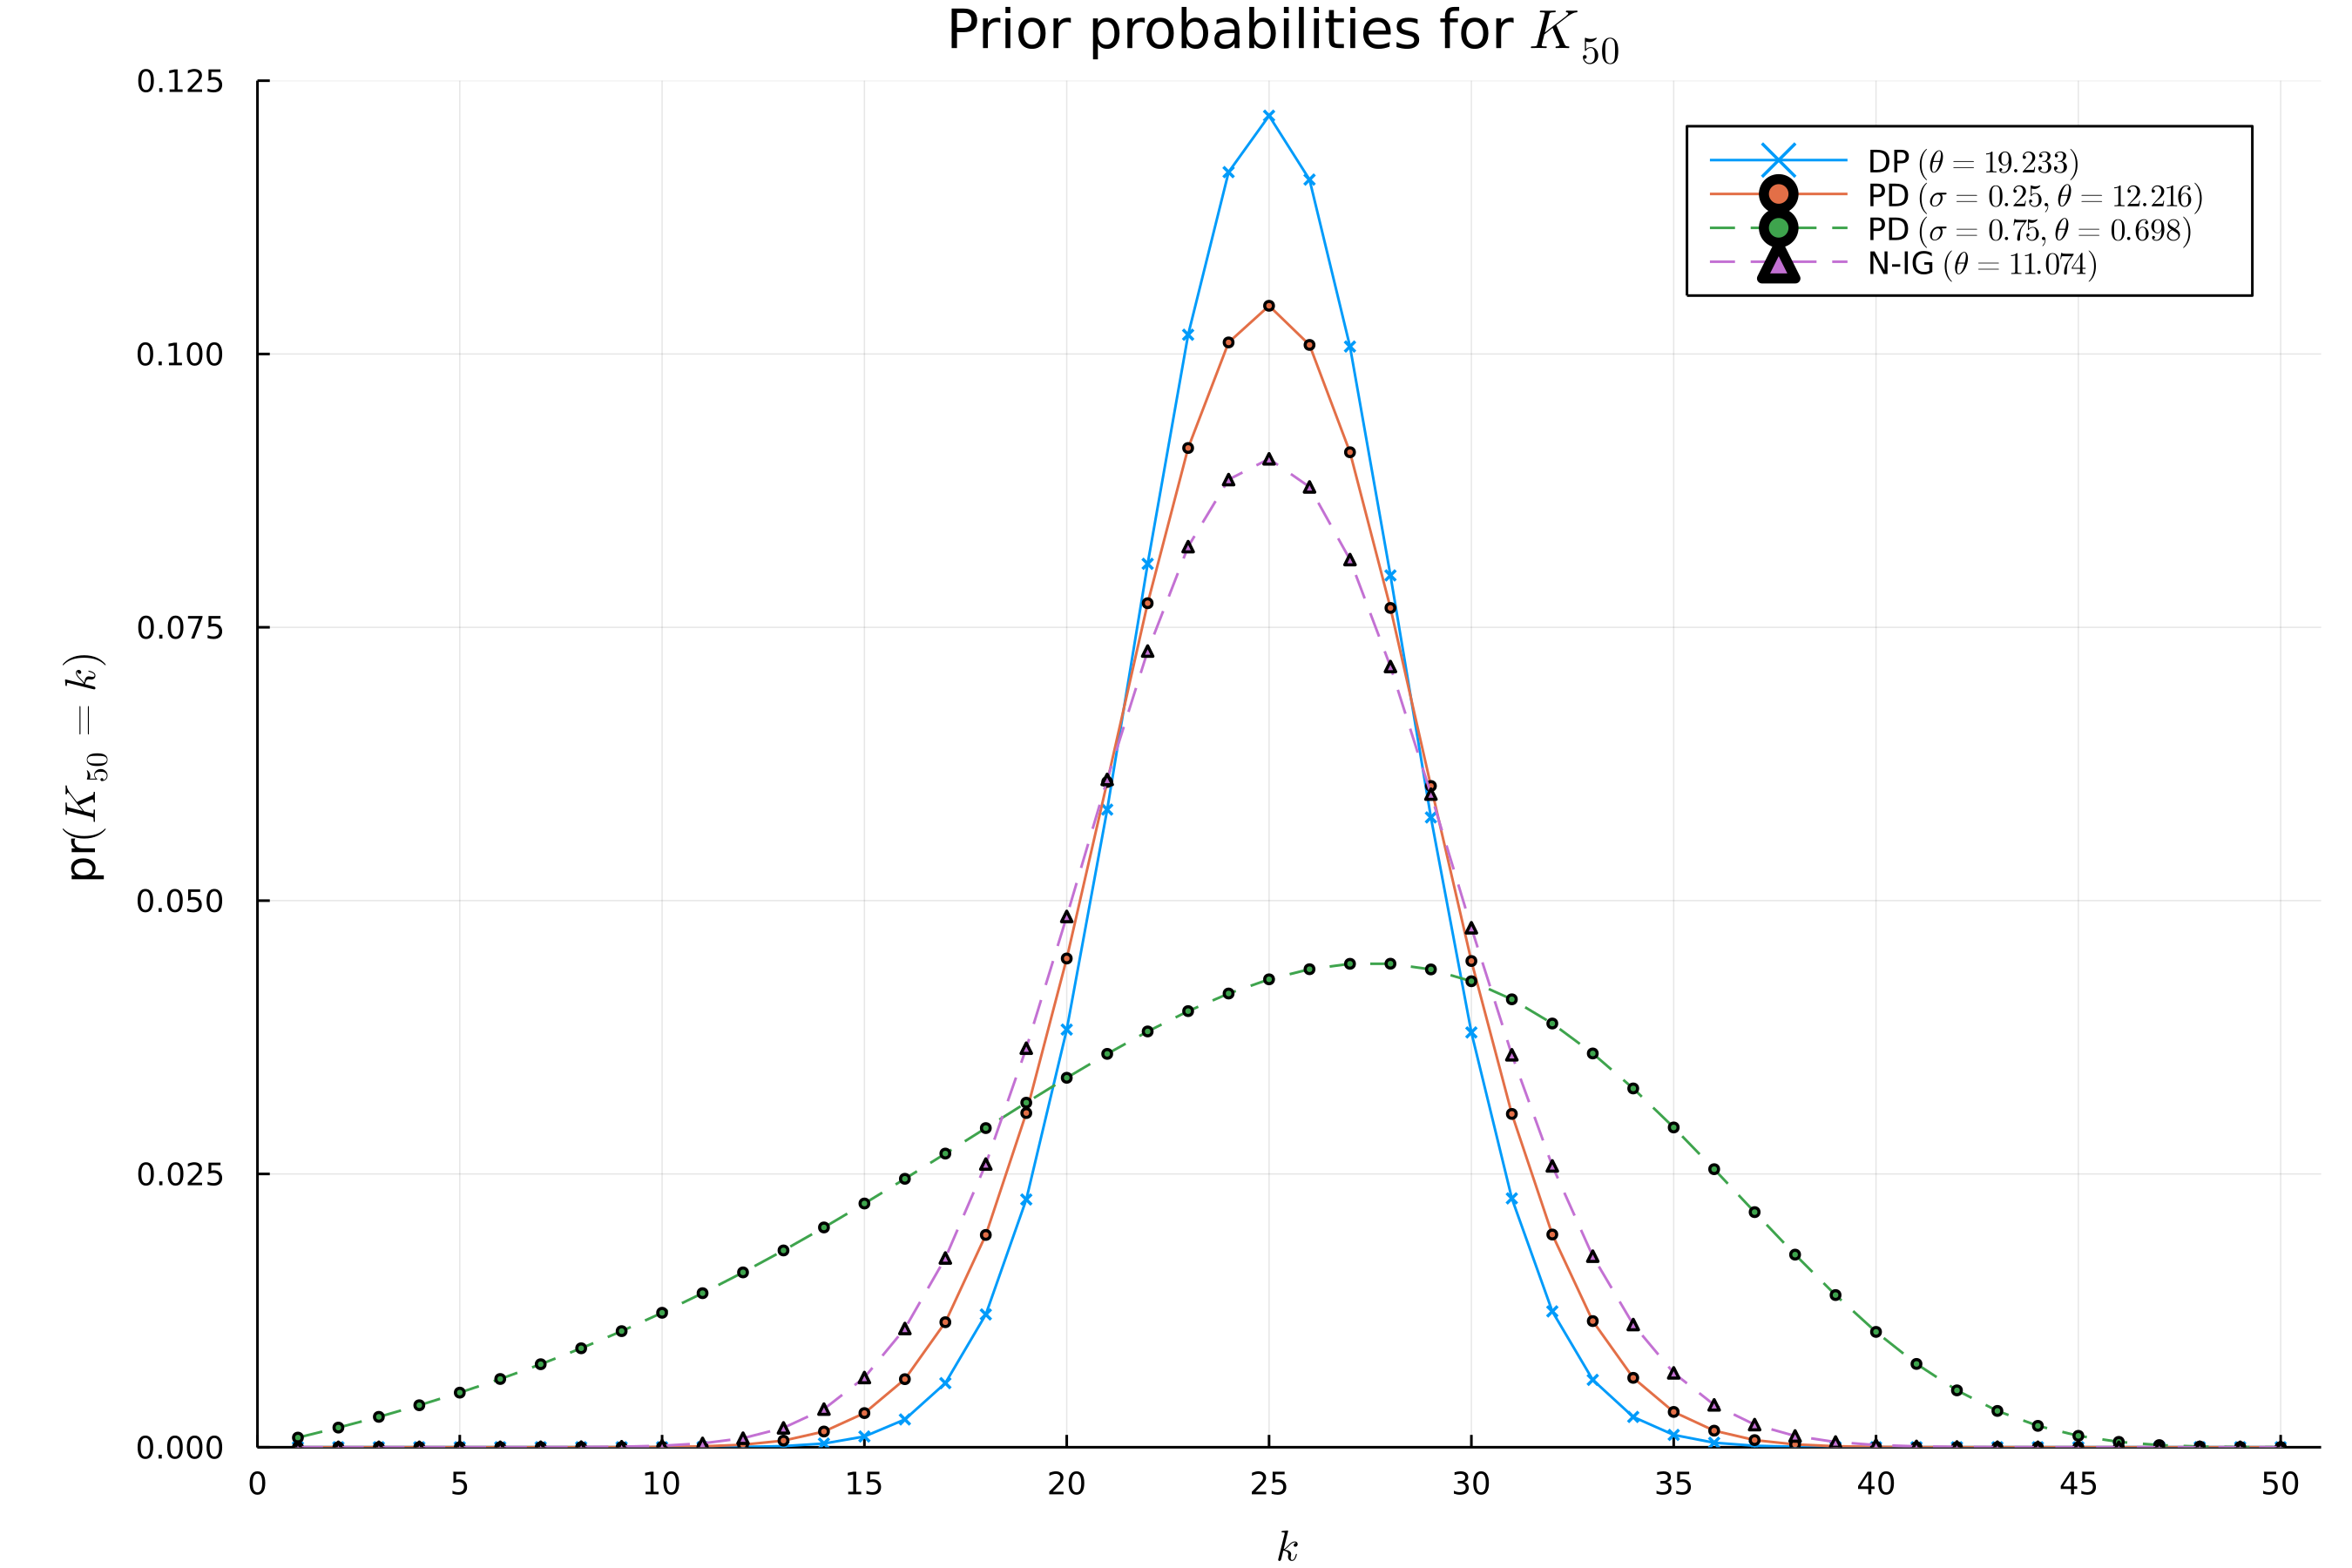
\includegraphics[scale=0.1]{../img/prior_probability.png}
        \caption{Prior probabilities of \(K_{50}\) corresponding to four different choices of Gibbs-type priors such that \(E(K_{50}) = 25\).}
        \label{fig:prior}
    \end{figure}
\end{frame}

\begin{frame}{Example - Posterior distribution} 
    % j \in {5, 25, 45} distinct species observed in first 50 observations
    % posterior probability of observing k species in additional dataset of size m = 50
    % not shown here, but, as m and n changes, behavior of prior relative to other choices doesn't change significantly
    % DP is inadequate due to independence from j
    % both PD and N-IG's posterior inferences are monotone in j
    % non-informative PD gives more weight to observed data
    \begin{figure}
        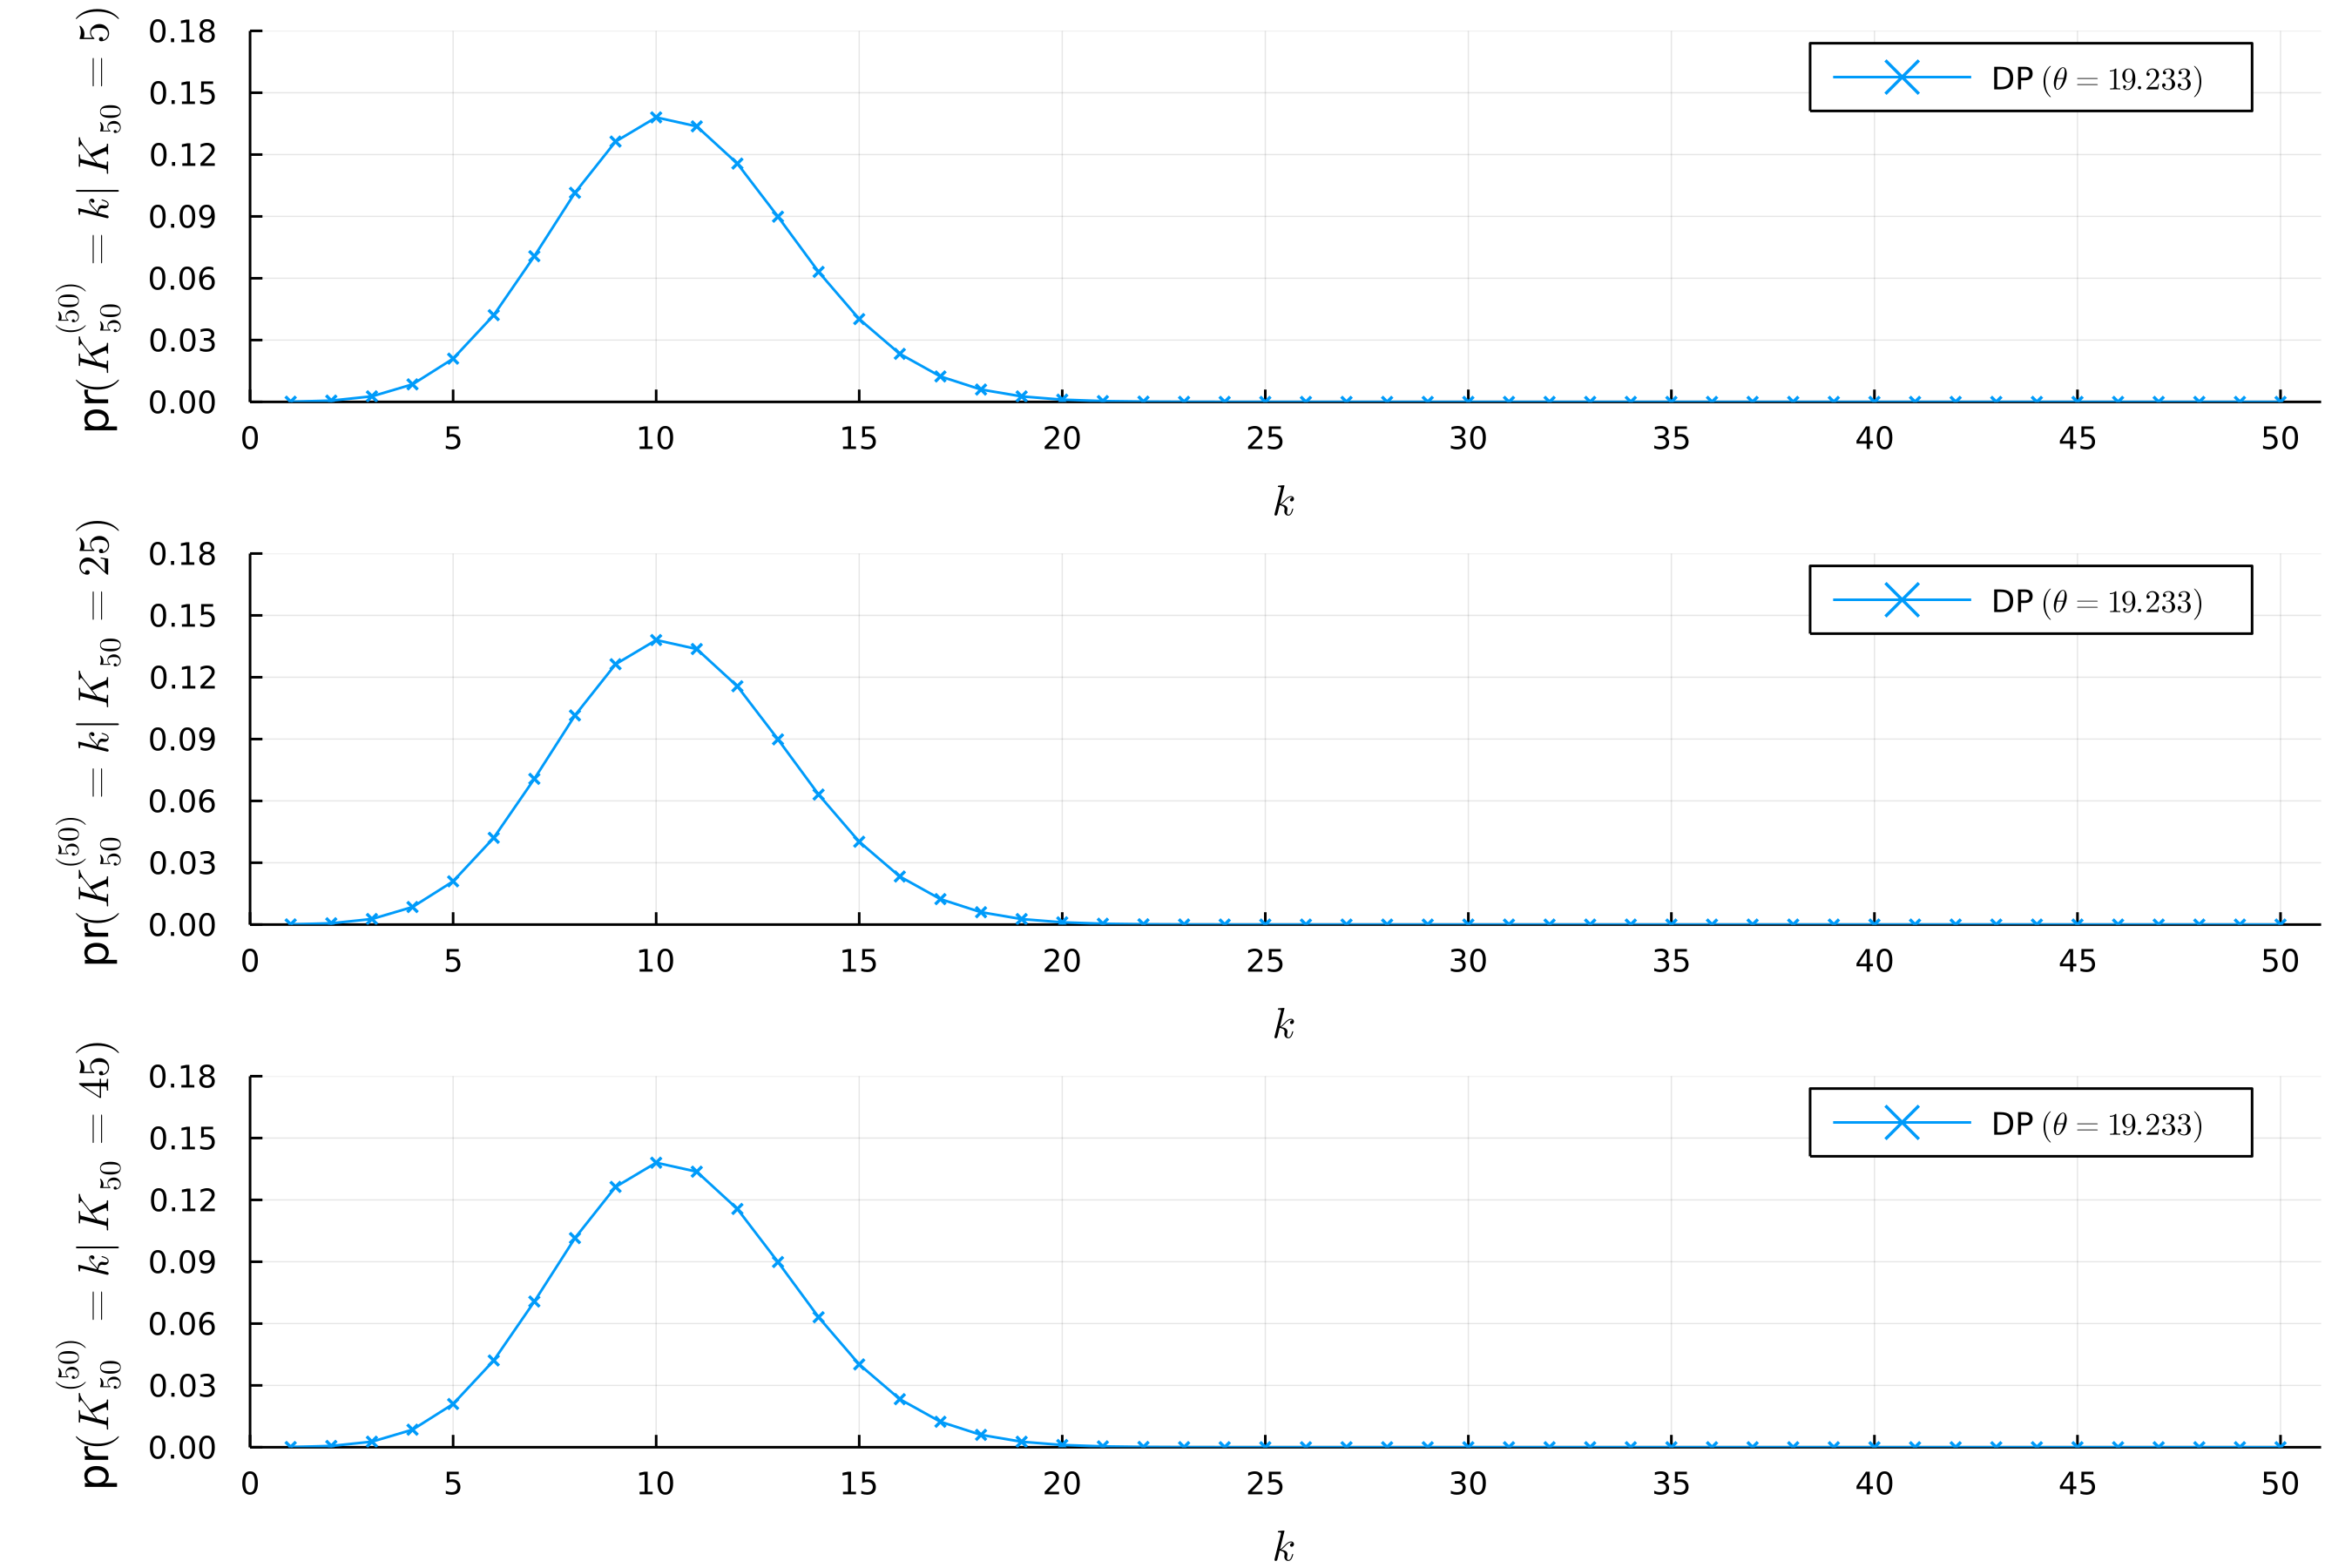
\includegraphics[scale=0.1]{../img/posterior_probability.png}
        \caption{Posterior probabilities of \((K^{(50)}_{50} | K_{50} = j)\) for \(j \in \{5, 25, 45\}\) corresponding to four different choices of Gibbs-type priors.}
        \label{fig:posterior}
    \end{figure}
        % table shows posterior mean and 95% highest posterior density intervals
\end{frame}

\section*{}
\begin{frame}{References}
    \scriptsize{\bibliographystyle{acm}}
    \bibliography{lijoi07}
\end{frame}
 
\end{document}